\section{Introduction}
Computing semantic relatedness(SR) between two words is a fundamental task for many applications in Natural Language
Processing(NLP) such as lexicon induction\cite{aaai/QadirMGL15}, Named Entity Disambiguation\cite{acl/HanZ10}, Keyword Extraction
\cite{ijcai/ZhangFW13} and Information Retrieval\cite{acl/GurevychMZ07}. Besides, in the aspect of spam problem\cite{www/SandulescuE15}
and image classification\cite{iwcs/LeongM11}, semantic relatedness measurement plays a great role as well.

Computing semantic relatedness between two words is to get a numerical value which indicates how related two words are.
In order to simulate the relatedness judgement of humans, many researchers have worked for semantic relatedness measurement and
have made great achievements. In the aspect of data resources for relatedness measurement, there are:
i) the methods based on \emph{lexical databases}\cite{acl/Pucher07,aaai/ZeschMG08,tkde/ZhuI17} mainly utilize fixed score functions, such as
the path information between two words or the nearest parent common node that two words hold in a lexical tree. These methods play a great part in
relatedness measurement and they employ precise and abundant lexical information, but miss the semantic information.
ii) \emph{the large corpus} based methods. WikiRelated\cite{aaai/StrubeP06}, ESA\cite{ijcai/GabrilovichM07}, WLM\cite{aaai/ZeschMG08}
and other methods exploit Wikipedia to compute semantic relatedness following co-occurrence principle, that is, two words
are related if they appear in fixed a window size or a sentence collectively. Experimental evaluation shows that these methods
outperform the lexical-based methods for the most part. Nevertheless, 1) in some special cases such as synonyms, two related words
hardly appear in a sentence. 2) the words that appear in the same sentence may not necessarily be closely related in their semantics
but co-occur by chance\cite{aaai/GongXH18}.

\begin{figure}
    \flushleft
    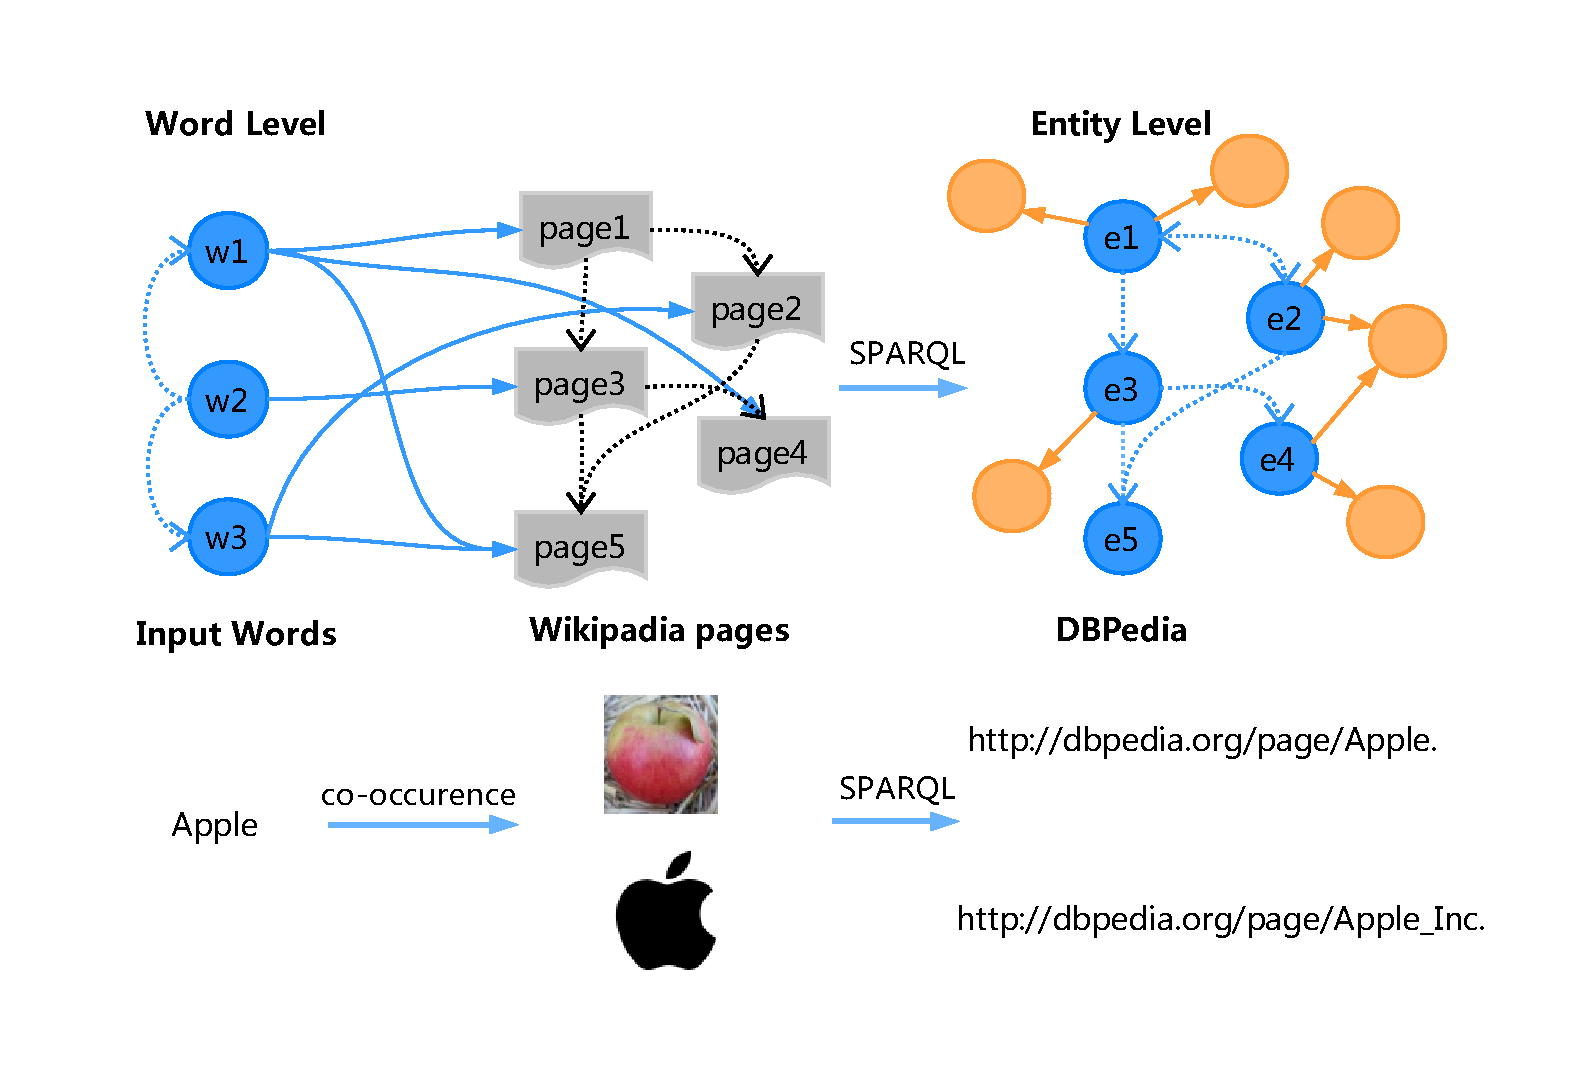
\includegraphics[width=0.5\textwidth]{pic/network.pdf}\\
    \caption{Knowledge Association Network}
    \label{network}
\end{figure}

To overcome the problems of co-occurrence principle, some approaches\cite{acl/IacobacciPN15,aaai/Pirro12} exploit latent semantic in knowledge graph.
Several of them utilize the special knowledge graph BabelNet\footnote{http://babelnet.org} to annotate different word senses
in dumps of Wikipedia, and the others regard that the predicates of triples are important features for words relatedness measurement in knowledge graph.
Recently, there are several approaches\cite{aaai/GongXH18,aaai/ZhangZH15} make great efforts based on the
\emph{free association process}\footnote{http://web.usf.edu/FreeAssociation/} in human mind. That is, when given a cue word, the first few words coming
into human mind are highly relevant to the cue word. These methods improve the weakness of co-occurrence based methods. However, when
comparing the concepts behind words, they mainly adopt some special score functions to judge the different aspects of concepts, such as
link information, co-occurrence times, categories of concepts, etc. These fixed functions cause lack of flexibility and
are less expressive than the distributed vector representation which is trained to optimize some loss functions. 
In addition, to get the structured information of concepts, they need significant preprocessing and data transformation efforts in Wikipedia.

In this paper, we use DBPedia and Wikipedia jointly where an entity corresponds to a title of Wikipedia page.
In this way we avoid the preprocessing of information extraction in Wikipedia, as DBPedia contains structured information extracted from Wikipedia.
Figure \ref{network} shows that, for a given word(\emph{apple}), there are some Wikipedia pages that contain this word(\emph{apple}),
and the titles of pages correspond to the entities in DBPedia. These entities and their relationships constitute the entities network,
where i) some relationships play a role of attributes(orange circles in figure \ref{network});
ii) some others just connect two entities without explicit semantic, such as two entities appear in the same Wikipedia page(blue circles),
which form the topological structure of entity network.
To get an approximation to human relatedness judgement more accurately,
we construct a knowledge association network to capture the relatedness of word-to-word, word-to-entity and
entity-to-entity. The contributions made in this paper include:

\begin{enumerate}
\item Based on the free association network, we propose a knowledge association network that is built on DBPedia which avoids the preprocessing in
Wikipedia and still keeps the complete semantics in our network.

\item For the relatedness measurement of entity-to-entity in our model, we use two different unsupervised methods to
represent the attributes and the topological structure of entity network rather than fixed score functions.
Finally we combine the relatedness of word-to-word, word-to-entity, entity-to-entity methodically.

\item We conduct experiments on standard dataset of semantic relatedness, and the result shows that our model gets
higher correlation coefficient than the state-of-the-art models.
\end{enumerate}

This paper is organized as follows. We give the definition and construction of knowledge association network firstly.
Then we elaborate the knowledge association network model to compute relatedness scores. Finally, we display detailed
illustrations of experiment results.